\documentclass{article}
\usepackage{amsmath}
\usepackage{xcolor}
\usepackage{gensymb}
\usepackage{ragged2e}
\usepackage{graphicx}
\usepackage{gensymb}
\usepackage{mathtools}
\newcommand{\mydet}[1]{\ensuremath{\begin{vmatrix}#1\end{vmatrix}}}
\providecommand{\brak}[1]{\ensuremath{\left(#1\right)}}
\providecommand{\norm}[1]{\left\lVert#1\right\rVert}
\newcommand{\solution}{\noindent \textbf{Solution: }}
\newcommand{\myvec}[1]{\ensuremath{\begin{pmatrix}#1\end{pmatrix}}}
\let\vec\mathbf
\begin{document}
\begin{center}
        \textbf\large{CHAPTER-7 \\ TRIANGLES}
\end{center}
\section{Exercise 7.1}
Q2. $ABCD$ is a quadrilateral in which $AD = BC$ and $\angle{DAB} = \angle{CBA}$ as shown in figure \ref{fig:Fig}. Prove that
\begin{enumerate}
\item $\triangle{ABD} \cong \triangle{BAC}$
  \item $BD = AC$
  \item $\angle{ABD} = \angle{BAC}$
\end{enumerate}
\textbf{Construction}\\
\begin{figure}[h!]
	\begin{center}
		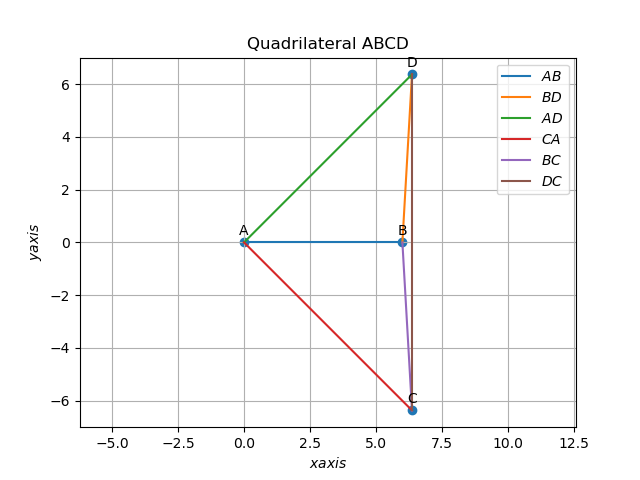
\includegraphics[width=\columnwidth]{figs/fig.png}
	\end{center}
	\caption{Quadrilateral ABCD}
	\label{fig:Fig}
\end{figure}
The input parameters for construction are shown in \ref{tab:Table1}:\\
\begin{table}[h!]
    \centering
    \begin{tabular}{|c|c|c|c|c|c|c|c|c|}                         
\hline & INPUT & \multicolumn{3}{|c|}{OUTPUT} & \multicolumn{2}{|c|}{CLOCK} & Vcc & GND     \\                                                                   
\hline ARDUINO & D6 & D3 & D4 & D5 &     \multicolumn{2}{|c|}{D2} & 5V & GND \\                              
\hline 7447 & & 5 & & & 3 & 11 & 14 & 7     \\                                                                 
\hline 7474 & 5 && 9 & 2 & \multicolumn{2}{|c|}{3} & 14 & 7 \\                                          
\hline                                     
\end{tabular}                   

    \caption{Parameters}
    \label{tab:Table1}
\end{table}
\pagebreak
\begin{align}
\vec{A} =& \myvec{0\\0},\vec{B} = \myvec{a\\0},\vec{C} = \myvec{c\cos\theta\\c\sin\theta},\vec{D} = \myvec{-c\cos\theta\\c\sin\theta}
\end{align}
\solution
\begin{align}
	\vec{A}-\vec{D} = \vec{B}-\vec{C}\\
  \angle{DAB} = \angle{CBA}
\end{align}
\textbf{To Prove:}
  \begin{align}
	  \triangle{ACB} &\cong \triangle{ADB}\\
	  BD &= AC\\
	  \angle{ABD} &= \angle{BAC}
  \end{align}
\textbf{Proof:}\\
In $\triangle{ABD}$ and $\triangle{BAC}$\\
Let  equation of $AB$ be $y = 0$, which can be written as:
\begin{align}
	\vec{n}^{\top}\vec{x} = 0,\\
\end{align}
\begin{align}
\vec{x} =& \myvec{x\\y},\vec{n} = \myvec{1\\0}\\
\end{align}
  From the above assumptions, we get the coordinates of $C$ and $D$ as
  \begin{align}
\vec{C} =& \myvec{4.3\\-2.5},\vec{D} = \myvec{-4.3\\-2.5}\\
  \end{align}
    Finding the angles(according to assumptions):
    \begin{align}
\text{Let }\theta_1=&\angle ADB\\
\vec{m_1}=&\vec{D}-\vec{A}=\myvec{-4.7\\-2.5}, \vec{m_2}=\vec{D}-\vec{B}=\myvec{-13.7\\-2.5}\\
\theta_1=&\cos^{-1}\frac{\vec{m_1}^\top\vec{m_2}}{\norm{\vec{m_1}}\norm{\vec{m_2}}}\\
\implies\theta_1=&\cos^{-1}\frac{\myvec{-4.7&-2.5}\myvec{-13.7\\-2.5}}{(9.2)(15.8)}=61\degree 
\label{eq:1}\\
\text{ Let }\theta_2=\angle ACB\\
\vec{n_1}=&\vec{C}-\vec{A}=\myvec{4.7\\-2.5}, \vec{n_2}=\vec{C}-\vec{B}=\myvec{13.7\\-2.5}\\
\theta_2 =& \cos^{-1}\frac{\vec{n_1}^\top\vec{n_2}}{\norm{\vec{n_1}}\norm{\vec{n_2}}}\\
\implies\theta_2=&\cos^{-1}\frac{\myvec{4.7&-2.5}\myvec{13.7\\-2.5}}{(9.2)(15.8)}=61\degree 
\label{eq:2}
\end{align}
from $\eqref{eq:1}$ and $\eqref{eq:2}$
\begin{center}
$\angle$ ABD = $\angle$ CAB \text{ (Sum of the angles in a triangle is 180\degree) }
\end{center}
Since all the angles and sides of triangles $CAB$ and $CAD$ are equal , from the definition of congruency both the triangles are said to be congruent to each other.
\begin{align}
    \triangle{ACB} & \cong \triangle{ADB}\\
    BD &= AC\\
    \angle{ABD} &= \angle{BAC}
\end{align}
\end{document}
